
\subsection*{\textbf{Question 5.b)}}
\begin{quote}

\textbf{Problem}
\begin{quote}
To check the robustness of your implementation make a plot of the x position of an individual particle and the value in cell 4 in 1 dimension and let x vary from the lowest value to the highest possible value in $x$. Repeat for cell 0.
\end{quote}

\textbf{Solution} 
\begin{quote}
There is not much to explain here, besides that the results for cell 4 and cell 0 are shown in the same plot. The code that creates the plot and the plot can be found below.

\end{quote}

\textbf{Code - Plots}
\begin{quote}
The code that creates the plots for cell 0 and cell 4. 
\lstinputlisting[firstline = 41, lastline=72]{./Code/assigment_5.py}
\end{quote}
\newpage

\textbf{Plots - Cell}
\begin{quote}
\begin{figure}[!ht]
\centering
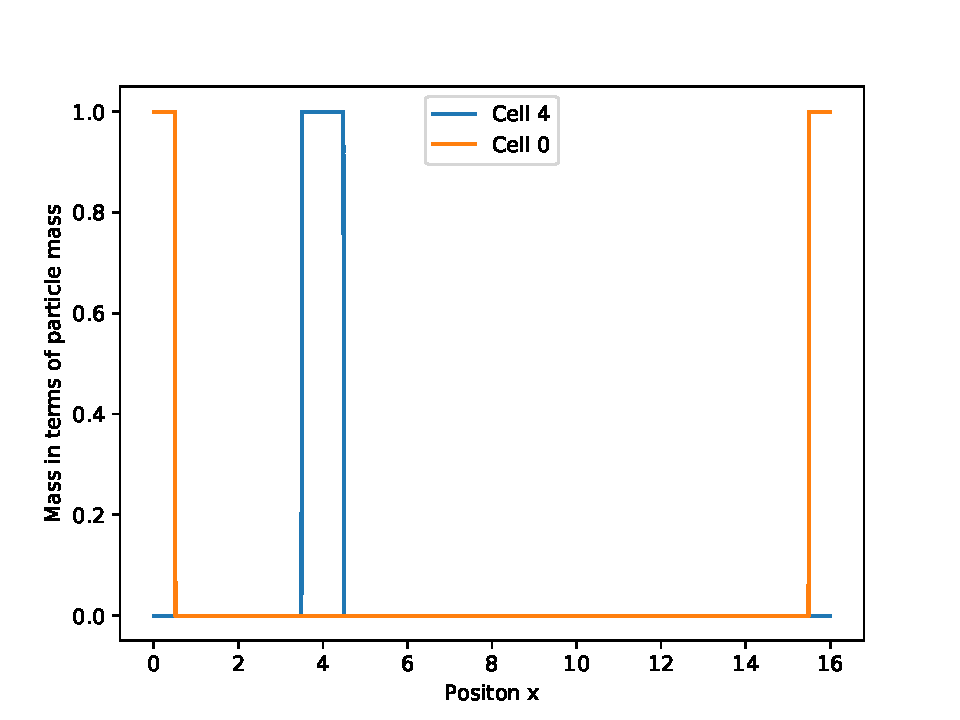
\includegraphics[width=14cm, height=8.5cm]{./Plots/5b_cell.pdf}
\caption{The mass assigned for a particle moving from x = 0 to x = 16. The orange and red line respectively indicate the mass assigned to cells 0 and 4 as function of the position of the particle. The plot is created for a mass grid of size 16 with circular boundary conditions.  }
\end{figure}

\end{quote}
\end{quote}











